\section{General architecture}
The structure of the project can be best described as an implementation of a multi-tier architecture consisting of the Translation Memory Core, the User Space and the web application GUI, as can be seen in Figure~\ref{projectStructure:layers}.

\begin{figure}[h]
\begin{center}
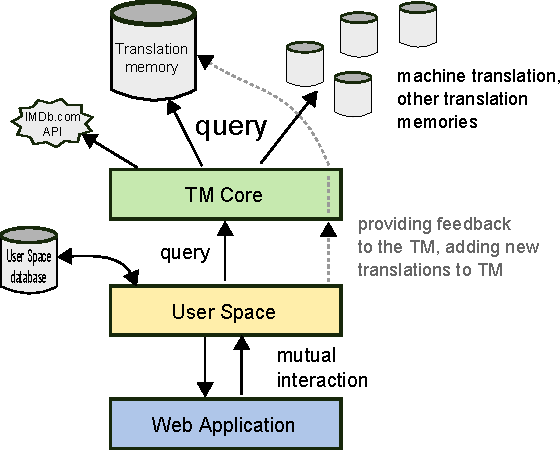
\includegraphics{figures/scheme.pdf}
\end{center}
\caption{Scheme of the application architecture.}\label{projectStructure:layers}
\end{figure}

\subsection*{TM Core}
The deepest level of the application is the \emph{Translation Memory Core}, which operates directly with the parallel chunks stored in the database. It is implemented in Scala. It provides an interface for retrieving translation suggestions from multiple sources -- different ways of processing our own translation memory and the machine translation output. It also assigns a score for each suggestion based on the retrieval parameters (e.g.\ edit distance for exact retrieval or term vector similarity in fuzzy retrieval) and movie characteristics taken from the \emph{Freebase.com} knowledge base.

The core layer also queries our machine translation server, which is running as a separate process and is using a phrase-based Moses translation engine.

\subsection*{Data import}

\emph{Data import} is a separate module, for cleaning up and parsing the data from the OpenSubtitles.org database, aligning language pairs and using the Core layer to import the pairs into the database. The classes should be run only once to have the data ready; however, we found it useful to have those data-importing classes as a part of the whole application, rather than some external scripts because it allowed us to repeatedly change the data themselves and keep the code compact. This part is also implemented in Scala.

\subsection*{User Space}

The middle-ware layer is called the User Space. Its task is to interact with the translation memory itself and mirror all GUI operations on the server side. The User Space is implemented in Java. It uses the same database as the Core and one database table is shared among them. The TM Core is used only as a service which is queried for translation suggestions. The interaction with the GUI is much more complicated because each operation from GUI has to be reflected in the US. The US provides a permanent storage of users' work to make the whole application including the users data available from the Internet. Except this function, the US provides the TM suggestion for the GUI.

\subsection*{GUI}

The GUI module is written in Java, using \emph{Google Web Toolkit}, which translates Java code into JavaScript and provides a framework for the simple implementation of remote procedure calls (RPCs) via the HTTP protocol, using POST requests. The server side of the GUI layer displays the appropriate JavaScript and CSS code to user's browser, which then communicates with the User Space through JavaScript AJAX calls through RPC, as is described above. The GUI lets the user log in, upload the subtitles, parses the subtitles into individual chunks, offers the user translations for every chunk and optionally plays the video of the chunks being translated.

\subsection*{Shared classes}

GUI and User Space are both written in Java (even when GUI is then translated to JavaScript) and can, therefore, have some Java \emph{shared classes}, which are used for communicating from the GUI to the User Space and from the User Space to the Translation Memory Core.


\subsection*{Other information}

Translation Memory Core and the User Space are both parts of the same \texttt{.jar} file and are, therefore, run in the same Java process. User Space is running as a Java Servlet.

The server side of the GUI, which returns the HTML, CSS and JavaScript, is also in the same \texttt{.jar} file, together with the required GWT assets, and is run as a second Servlet. There is also a third servlet which is used for downloading the exported subtitles.

All Servlets are loaded using a \emph{Jetty} web server. Maven is used for building the application and retrieving dependencies, the Jenkins tool was used for continuous building and testing of the project.

As noted above, a Moses machine translation server is running as a completely separate process.
%, and it is actually running on a completely separate computer.


\section{Sharing the Implementation among the Project}

Because all parts of the projects are Java based, we can share a set of classes between the GUI and the server to avoid unnecessary redundancy and to make the project structure clearer.

However, as noted in the GWT documentation,\footnote{\url{https://developers.google.com/web-toolkit/doc/latest/DevGuideCodingBasicsCompatibility} and \url{https://developers.google.com/web-toolkit/doc/latest/RefJreEmulation}} not all Java classes are directly translatable to GWT. The main issues we encountered were:

\begin{itemize}
\item The shared classes cannot reference any class that is not translatable to JavaScript through GWT (for example, any third-party libraries).
\item The shared classes can use only a subset of the Java Runtime Library. E.g. we could not use \texttt{java.util.regex}, which is not implemented in GWT; we had to use \texttt{com.google.gwt.regexp.shared} instead.
% I dont think this was the main case, there were more such cases...
\item Serialization works differently in GWT. What this effectively meant for us is that, even when we use the general \texttt{List} interface for a property, we cannot set the value to an instance of a subtype of \texttt{List} that is not implemented in GWT. More specifically -- we wanted to use \texttt{scala.collection.JavaConverters.AsJava[List]} for Scala $\Leftrightarrow$ Java conversion, but it was not possible, since it uses its own implementation of Java \texttt{List} interface.
\end{itemize}

Therefore, shared classes could only use a subset of Java. Generally, what is translatable with GWT to JavaScript is also translatable by the Java compiler to JVM bytecode (except for direct insertions of Javascript code of course), but not the other way around.

Structure of the shared classes follows the terms mentioned in the Glossary as can be seen in Figure~\ref{projectStructure:logical}. Detailed UML diagram of the shared classes is in Figure~\ref{fig:shared_uml} and Figure~\ref{fig:shared_uml_helping}.


\begin{figure}[h]
\begin{center}
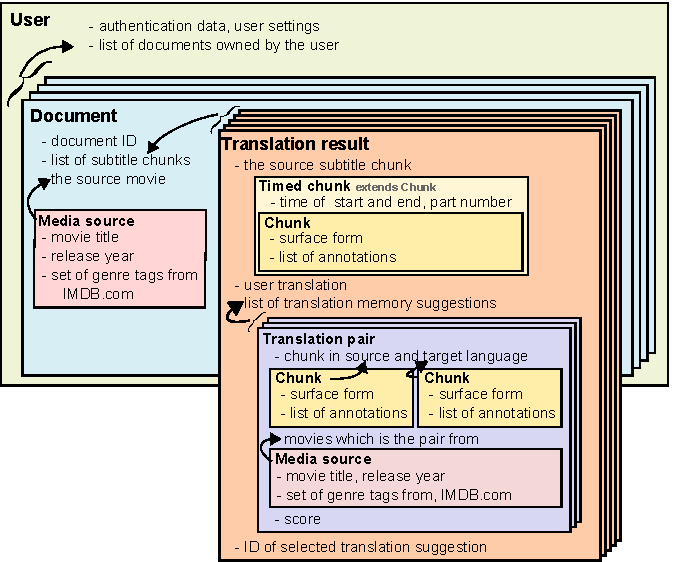
\includegraphics{figures/shared_classes.pdf}
\end{center}
\caption{Scheme of the shared classes.}\label{projectStructure:logical}
\end{figure}

\begin{figure}
\begin{center}
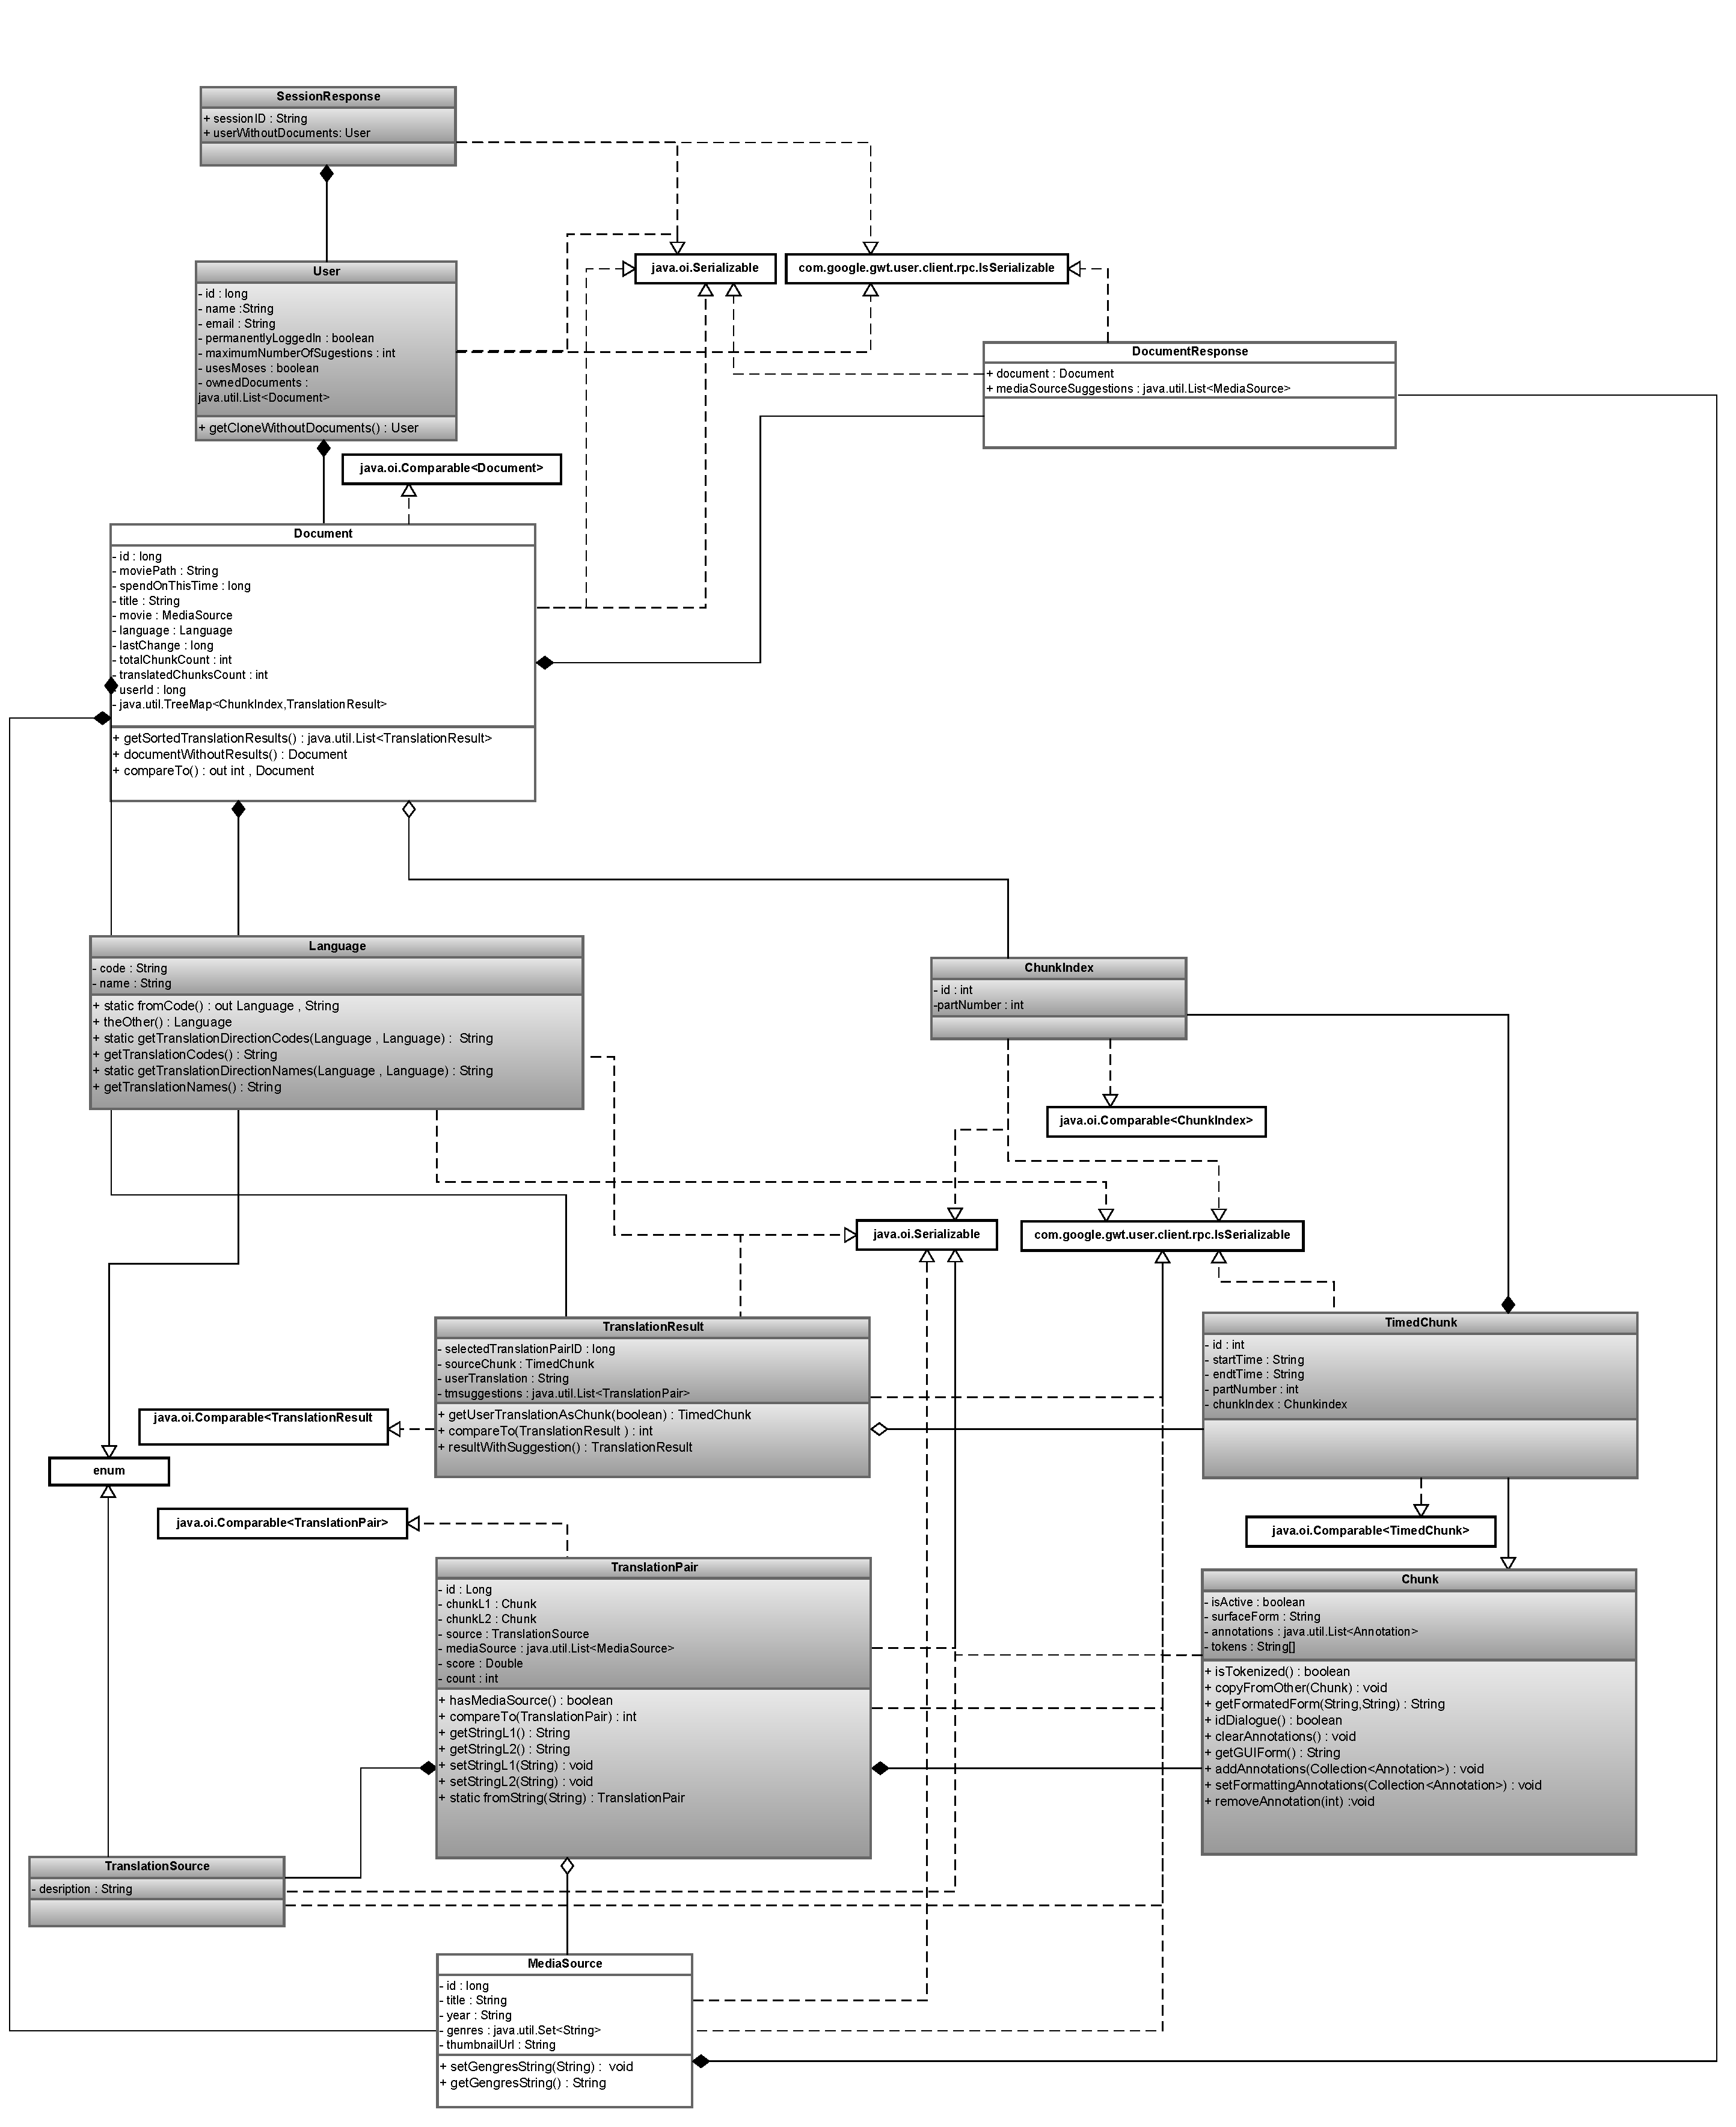
\includegraphics[scale=0.38]{figures/shared.pdf}
\end{center}
\caption{UML diagram of shared classes}
\label{fig:shared_uml}
\end{figure}

\begin{figure}
\begin{center}
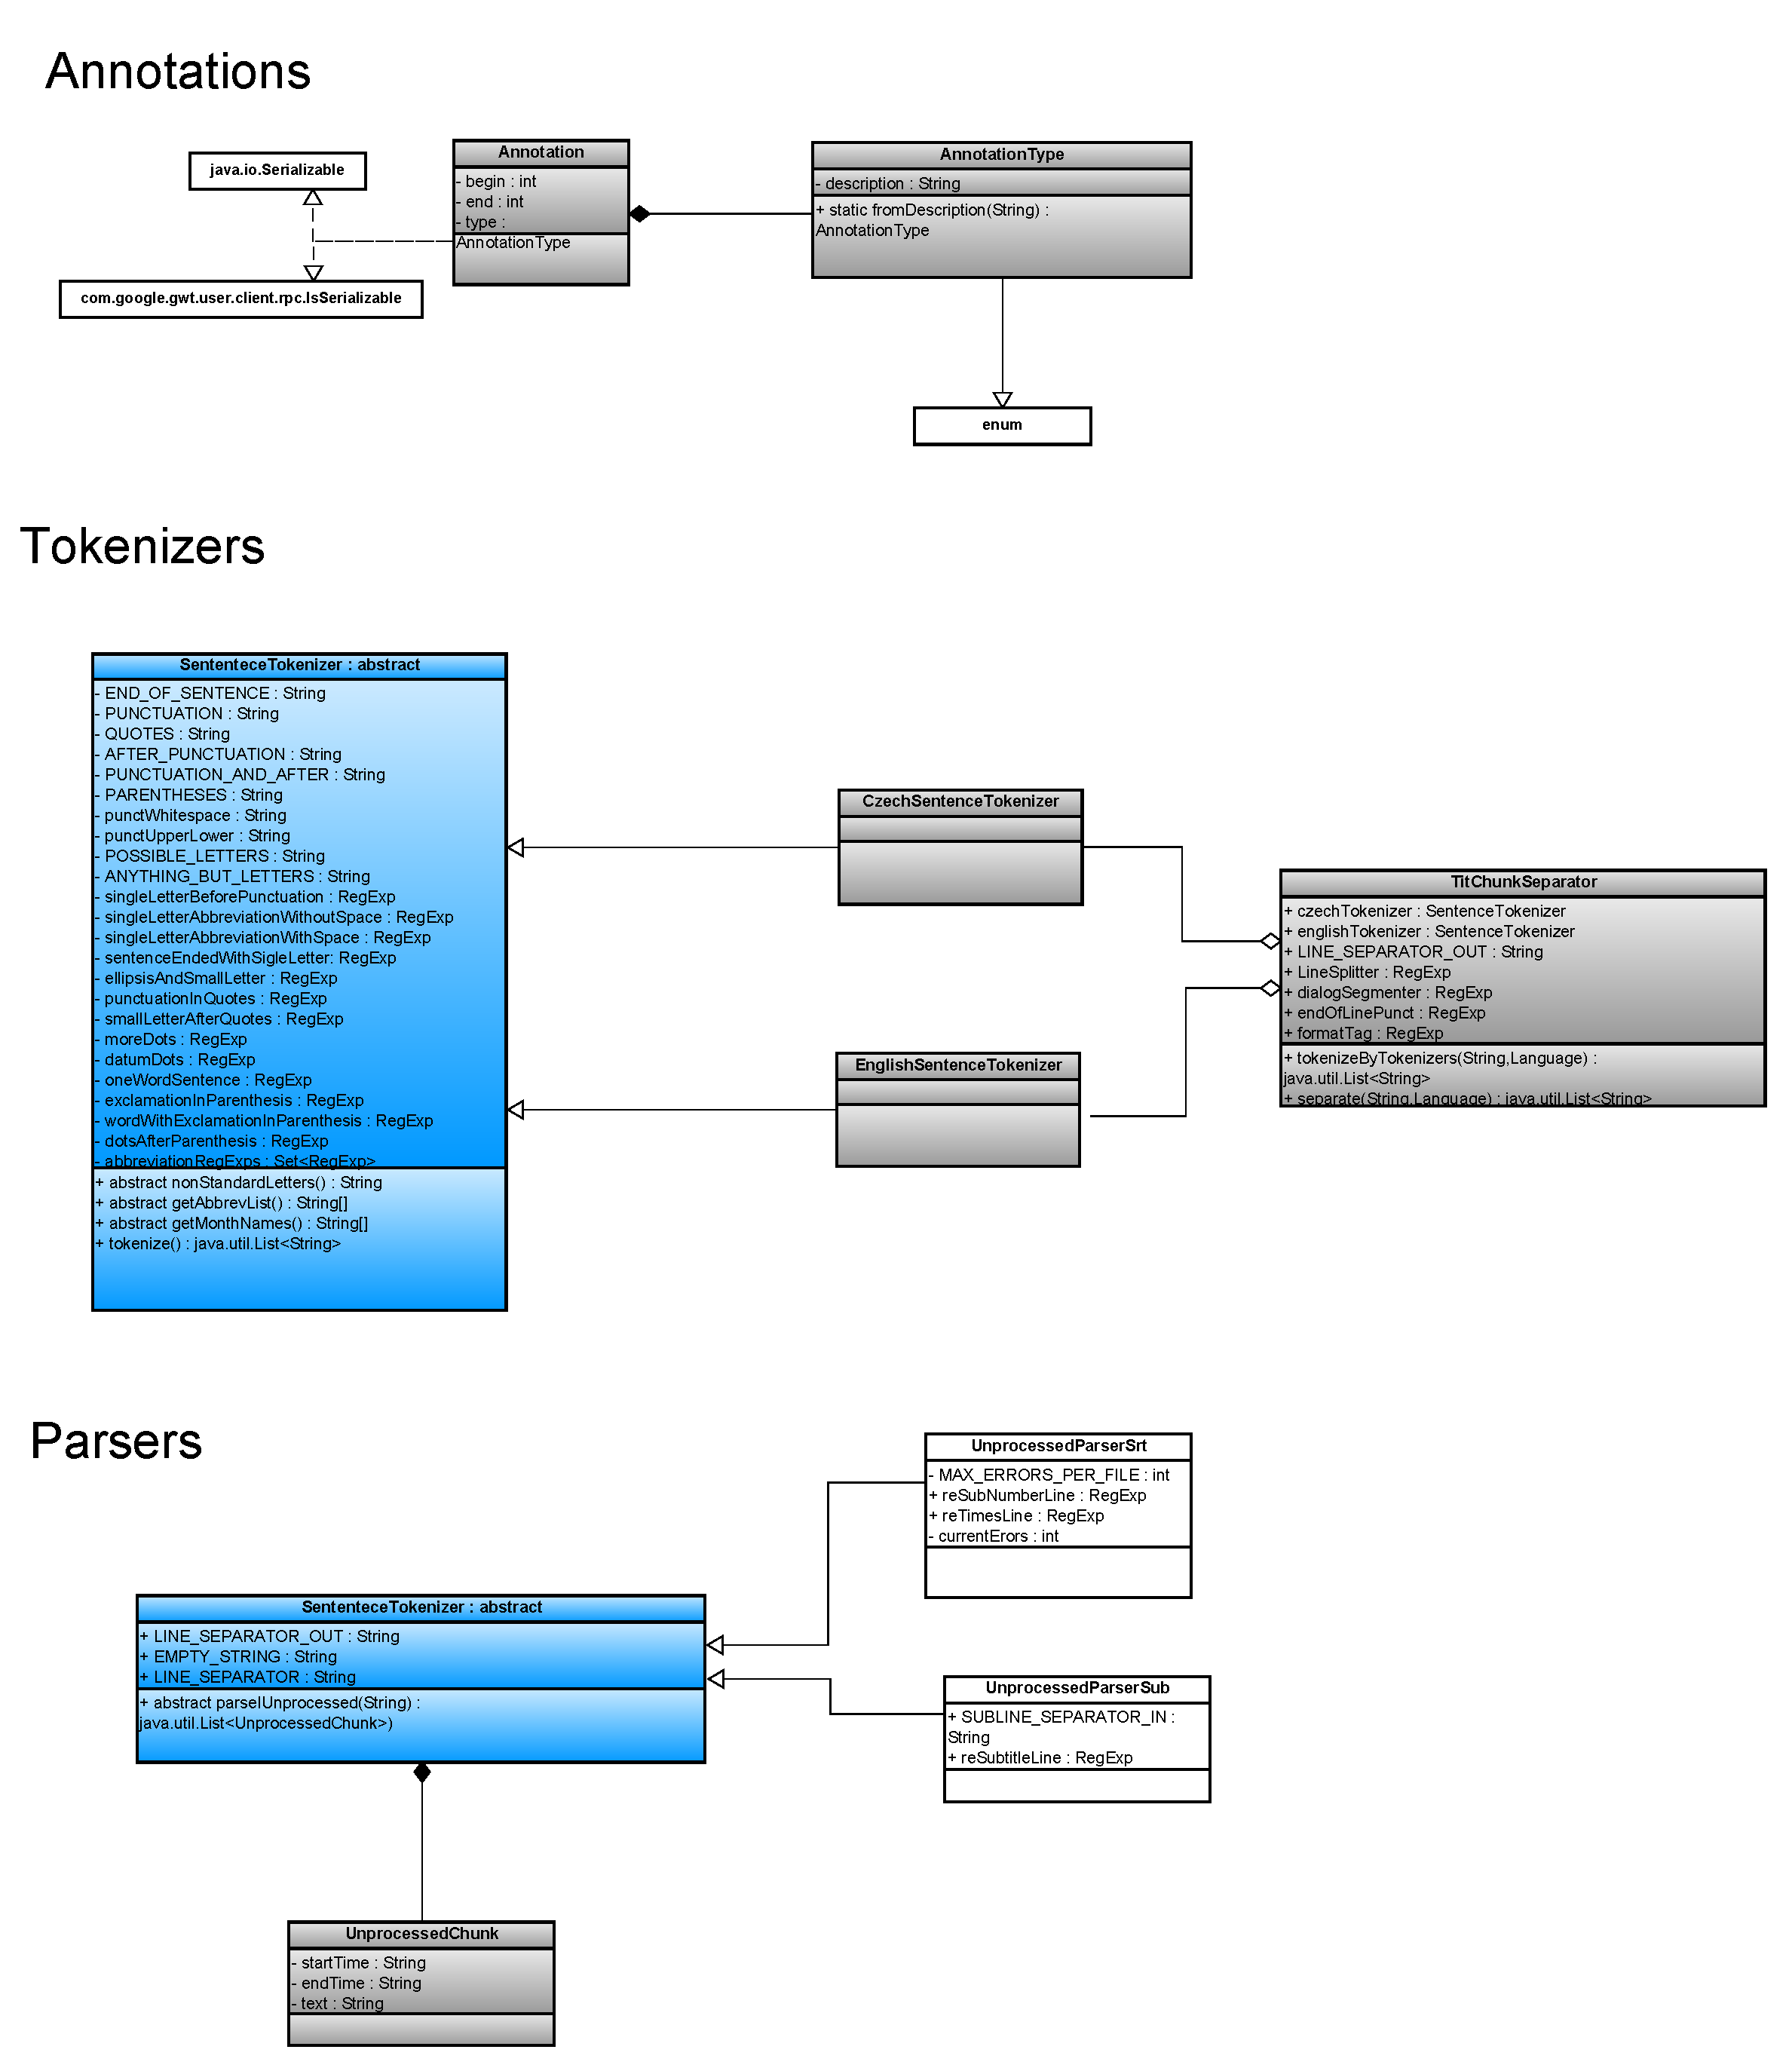
\includegraphics[scale=0.38]{figures/shared2.pdf}
\end{center}
\caption{UML diagram of helping shared classes providing functionality needed among different modules}
\label{fig:shared_uml_helping}
\end{figure}

\section{Usage of Third Party Libraries}

We use a number of third party libraries and tools. Most of them are linked to the project as Maven dependencies. An overview of the used dependencies including their licenses and a short descriptions is provided below.

\begin{itemize}
\item {\bf Scala Compiler 2.9.1} -- Scala License \\
Compiler of the Scala programming language.
\item {\bf Posgres SQL 9.1.} -- PosgreSQL License (similar to MIT and BSD lincences) \\
The JDBC driver allowing the application to connect to a PostgreSQL database.
\item {\bf Google Web Toolkit 2.4.0} -- Apache License 2.0 \\
Google Web Toolkit is an open source set of tools that allows web developers to create and maintain complex JavaScript front-end applications in Java.

\item {\bf Hibernate Validator 4.1.0.Final} -- Apache License 2.0 \\
Hibernate Validator is the reference implementation for JSR 303 - Bean Validation. Bean Validation defines a metadata model and API for JavaBean validation.

\item {\bf JUnit 4.10} -- Common Public License, v 1.0 \\
JUnit is a unit testing framework for the Java programming language.

\item {\bf ScalaTest 1.6.1} -- Apache License 2.0 \\
ScalaTest is a unit testing framework for both Scala and Java programming languages.

\item {\bf language-detection} -- Apache License 2.0 \\
This is a language detection library implemented in plain Java developed by the Cybozu company.

\item {\bf Apache XML-RPC client} -- Apache License 2.0  \\
An implementation of XML-RPC, a remote procedure call protocol which uses XML to encode its calls and HTTP as a transport mechanism.

\item {\bf Apache Commons} -- Apache License 2.0 \\
The Apache Commons is a project of the Apache Software Foundation, formerly under the Jakarta Project. The purpose of the Commons is to provide reusable, open source Java software. We use particularly the Lang3, Math and Validator components.

\item {\bf OpenNLP 1.5.2} -- Apache License 2.0 or LGPL \\
The Apache OpenNLP library is a machine learning based toolkit for the processing of natural language text. It supports the most common NLP tasks, such as tokenization, sentence segmentation, part-of-speech tagging, named entity extraction, chunking, parsing, and coreference resolution. These tasks are usually required to build more advanced text processing services.

\item {\bf HSQLDB 2.2.8} -- BSD License \\
HSQLDB (Hyper Structured Query Language Database) is a relational database management system written in Java. It can be used just in the memory. (Used in tests.)

\item {\bf Google Guava 11.0.2} -- Apache License 2.0 \\
The Guava contains several of Google's core libraries: collections, caching, primitives support, concurrency libraries, common annotations, string processing, I/O, and so forth.

\item {\bf Jetty Sever 7.2.0} -- Apache License 2.0 or Eclipse Public Licence 1.0 \\
Jetty is a pure Java-based HTTP server and Java Servlet container. Jetty is developed as a free and open source project as part of the Eclipse Foundation.

\item {\bf Trove4j 3.0.2} -- LGPL 2.1 \\
The Trove library provides high speed regular and primitive collections for Java. 

\item {\bf Lorem Ipsum For Java} -- MIT License \\
The Lorem Ipsum dummy text generator for Java. (Used in tests.)

\item {\bf JSON 20090211} -- JSON License (similar to MIT and BSD licences)

\item {\bf Apache log4j 1.2.16}  -- Apache License 2.0 \\
Apache log4j is a Java-based logging utility.

\item {\bf Simple Logging Facade for Java 1.6.4} -- MIT License \\
The Simple Logging Facade for Java or (SLF4J) serves as a simple facade or abstraction for various logging frameworks, e.g. java.util.logging, log4j and logback, allowing the end user to plug in the desired logging framework at deployment time.

\item {\bf Hibernate ORM 4.1.0} -- LGPL 2.1 \\
Hibernate is an object-relational mapping library for the Java language, providing a framework for mapping an object-oriented domain model to a traditional relational database.

\item {\bf Akka 2.0.1} -- Apache License 2.0 \\
Actors are very lightweight concurrent entities. They process messages asynchronously using an event-driven receive loop. Pattern matching against messages is a convenient way to express an actor's behavior. They raise the abstraction level and make it much easier to write, test, understand and maintain concurrent and/or distributed systems. You focus on workflow, how the messages flow in the system, instead of low level primitives like threads, locks and socket IO.
 
\item {\bf JOpenID 1.08} -- Apache License 2.0 \\
JOpenID is an OpenID 2.0 Java 5 implementation for OpenID sign on.

\item {\bf LiftWeb 2.4} -- Apache License 2.0 \\
Lift is a free web application framework that is designed for the Scala programming language. It JSON library is used in this project.

\item {\bf Weka} -- GPL 2.0\\
Weka (short for \emph{Waikato Environment for Knowledge Analysis}) is a machine learning software that we use to train and apply machine learning models for ranking translation pair candidates.
\end{itemize}

We also directly use code from other libraries. These are:

\begin{itemize}
\item {\bf IdGenerator} from Direct Web Remoting -- Apache License 2.0\\
IdGenerator is a class for generating session IDs.

\item {\bf BCrypt} -- BSD License\\
We use BCrypt for saving the passwords to the database.

\item {\bf LanguageTools} -- LGPL 2.1\\
Our rule-based sentence splitter is based on LanguageTools' SentenceTokenizer.

\end{itemize}

\subsection*{Licenses}
Most of the licenses are non-permissive and would allow us to publish our code with a non-permissive license, e.g.\ Apache License 2.0, if we wanted to do so.

However, two libraries are a problem -- Weka, that uses GPL, and LanguageTools, which use LGPL, but we use its code directly.

To satisfy the licensing requirements, we need to license our code in a license compatible with GPL 2.0. It would be a very manageable amount of work to replace the two problematic libraries and license the whole project under a non-permissive license.